\documentclass{article}
\usepackage[catalan]{babel}
\usepackage[latin1]{inputenc}   % Permet usar tots els accents i car�ters llatins de forma directa.
\usepackage{enumerate}
\usepackage{amsfonts, amscd, amsmath, amssymb}
\usepackage[pdftex]{graphicx}

\setlength{\textwidth}{16cm}
\setlength{\textheight}{24.5cm}
\setlength{\oddsidemargin}{-0.3cm}
\setlength{\evensidemargin}{0.25cm} \addtolength{\headheight}{\baselineskip}
\addtolength{\topmargin}{-3cm}

\newcommand\Z{\mathbb{Z}}
\newcommand\R{\mathbb{R}}
\newcommand\N{\mathbb{N}}
\newcommand\Q{\mathbb{Q}}
\newcommand\K{\Bbbk}
\newcommand\C{\mathbb{C}}

\newcounter{exctr}
\newenvironment{exemple}
{ \stepcounter{exctr} 
\hspace{0.2cm} 
\textit{Exemple  \arabic{exctr}: }
\it
\begin{quotation}
}{\end{quotation}}


\begin{document}

\textbf{\Large Tema 2.Sistemes}

\vskip 0.3 cm
\noindent
S'anomena \textbf{sistema} a qualsevol dispositiu o algoritme que modifica un senyal (entrada) 
per obtenir-ne un nou senyal (sortida) seguint alguna regla ben definida
(\'es a dir, no es tracta d'una modificaci\'o aleat\`oria del senyal).

\vskip 0.2 cm
\noindent
\textbf{Notaci\'o}. Per denotar que un sistema ${\cal T}$ transforma un senyal d'entrada $x$ 
en un senyal de sortida $y$ ho podem fer de 3 maneres:

\vskip 0.2 cm
\begin{center}
\begin{tabular}{ccccc}
1) 
\begin{minipage}{5cm}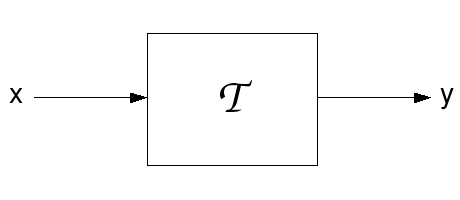
\includegraphics[width=5cm]{notaciosistema.png}\end{minipage} & &
2) $x \xrightarrow{{\cal T}} y $ & & 3) $y={\cal T}(x)={\cal T} \, x$ \\
(diagrama de blocs) & & & & 
\end{tabular}
\end{center}
\vskip 0.2 cm


\vskip 0.2 cm
\noindent
Exemples de sistemes:
\begin{itemize}
\item Acumulador

\begin{tabular}{lr}
$y[n]=y[n-1]+x[n]$ &
\begin{minipage}{5cm}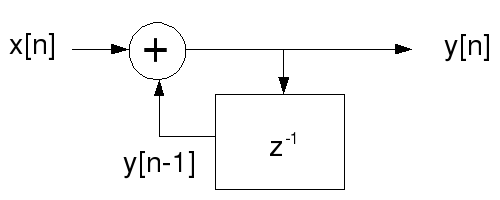
\includegraphics[width=5cm]{acumulador.png}\end{minipage}
\end{tabular}

\vskip 0.2 cm
\noindent
De manera equivalent es pot escriure: $y[n]=\sum_{k=-\infty}^n x[k]$

\item Diferenciador

\begin{tabular}{lr}
$y[n]=x[n-1]-x[n]$ &
\begin{minipage}{5cm}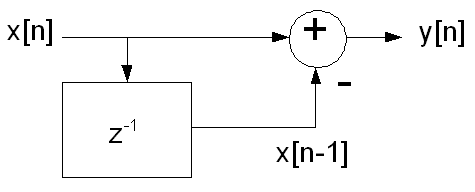
\includegraphics[width=5cm]{diferenciador.png}\end{minipage}
\end{tabular}

\item $y[n]=\mathrm{max}(x[n], x[n-1])$

\end{itemize}

\vskip 0.3 cm
\noindent
\textbf{Classificaci\'o dels sistemes}
\begin{itemize}

\item Sistemes lineals i no lineals.
Un sistema ${\cal T}$ es diu \textbf{lineal} si verifica que
\[
{\cal T}(ax_1[n]+bx_2[n])=a {\cal T}(x_1[n]) + b {\cal T}(x_2[n])
\]
\noindent
per a qualsevol parell de senyals d'entrada $x_1[n]$ i $x_2[n]$ i qualssevol
escalars $a$ i $b$.

\noindent
Si un sistema ${\cal T}$  \'es lineal llavors els seg\"uents diagrames de blocs 
s\'on equivalents:

\vskip 0.2 cm
\begin{center}
\begin{tabular}{ccc}
\begin{minipage}{6cm}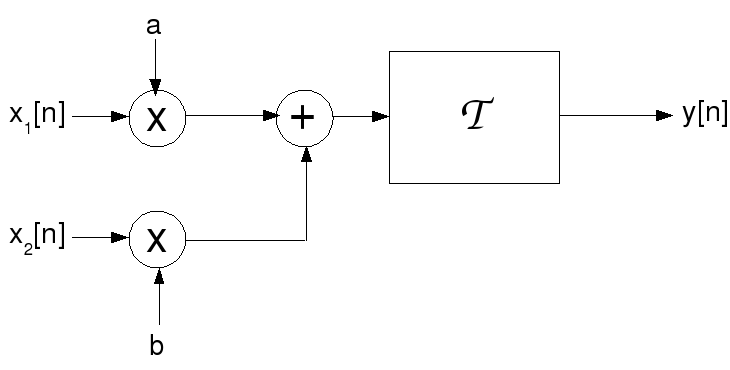
\includegraphics[width=6cm]{lineal1.png}\end{minipage}
 & $\qquad$ &
\begin{minipage}{6cm}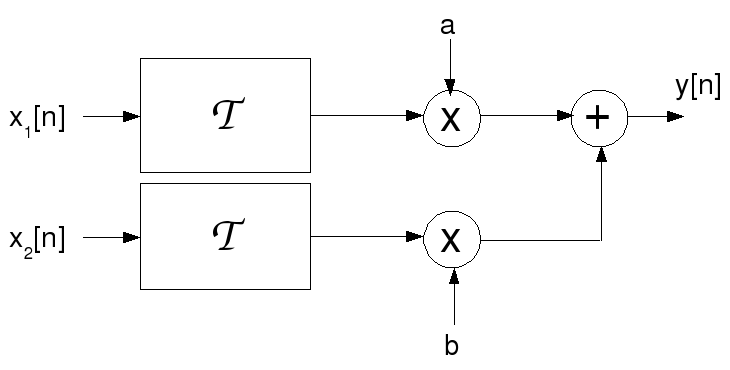
\includegraphics[width=6cm]{lineal2.png}\end{minipage}
\end{tabular}
\end{center}


\noindent
Exemples:
\begin{center}
\begin{tabular}{|c|c|}
 lineals & no lineals \\ \hline
$y[n]=Ax[n]$ & $y[n]=Ax[n]+B$ \\ & \\
$y[n]=nx[n]$ & $y[n]=nx[n]+B$ \\ & \\
$y[n]=x[n^2]$  & $y[n]=x^2[n]$ \\ & \\
$y[n]=e^n x[n]$ & $y[n]=e^{x[n]}$
\end{tabular}
\end{center}

\vskip 0.2cm
\noindent
Propietat dels sistemes lineals (\textbf{principi de superposici\'o}):
\[
{\cal T}(\sum_{k=1}^M a_k x_k[n]) =  \sum_{k=1}^M a_k y_k[n]
\]
\noindent
on $y_k[n]={\cal T} x_k[n]$, $(k=1, \cdots, M$.


\item Sistemes variants i invariants en el temps.
Un sistema es diu \textbf{invariant en el temps} si
a una entrada retardada en el temps li correspon una
sortida amb el mateix retard temporal. \'Es a dir:
\[
\text{si } y[n]={\cal T}(x[n]) \qquad \text{llavors} \qquad
y[n-k]={\cal T}(x[n-k])
\]

\noindent
Si un sistema ${\cal T}$  \'es invariant en el temps llavors els seg\"uents diagrames de blocs 
s\'on equivalents:

\vskip 0.2 cm
\begin{center}
\begin{tabular}{ccc}
\begin{minipage}{6cm}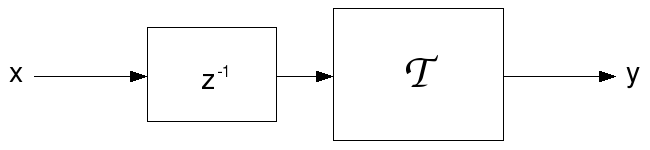
\includegraphics[width=6cm]{tinvariant1.png}\end{minipage}
 & $\qquad$ &
\begin{minipage}{6cm}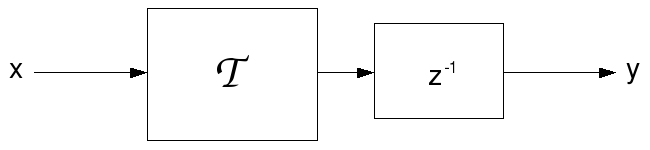
\includegraphics[width=6cm]{tinvariant2.png}\end{minipage}
\end{tabular}
\end{center}

\noindent
Exemples:
\begin{center}
\begin{tabular}{|c|c|}
 invariants en temps & no invariants \\ \hline
 $y[n]=x[n]-x[n-1]$ & $y[n]=nx[n]$  \\ & \\
 $y[n]=Ax[n]+B$ &  $y[n]=x[-n]$
\end{tabular}
\end{center}

\item Sistemes causals i no causals. Un sistema es diu \textbf{causal} si la seva
sortida en l'instant $n$ no depen de les entrades en els instants de temps
$n+1, n+2, \cdots$.

\noindent
Exemples:
\begin{center}
\begin{tabular}{|c|c|}
 causals & no causals \\ \hline
$y[n]=x[n]+x[n-5]$ & $y[n]=x[n]+x[n+5]$ \\ & \\
$y[n]=ax[n]$  & $y[n]=ax[-n]$ \\ & \\
$y[n]=x^2[n]$ & $y[n]=x[n^2]$ \\ & \\
$y[n]=3x[n]$ & $y[n]=3x[2n]$
\end{tabular}
\end{center}

\vskip 0.2 cm
\noindent
\textbf{Observaci\'o}: en sistemes que treballen en temps real 
(el processament es fa a mida que arriben els senyals d'entrada)
no \'es possible con\`eixer els valors futurs de l'entrada, per la qual cosa 
aquest sistemes nom\'es poden \'esser causals.

\item Sistemes estables i inestables.
Un sistema es diu \textbf{estable} si d\'ona sortides fitades a
entrades fitades.

\noindent
Exemples:
\begin{center}
\begin{tabular}{|c|c|}
 estables & inestables \\ \hline
$y[n]=ax[n]$ & $y[n]=\sum_{k=0}^\infty x[n-k]$ \\ & \\
$y[n]=\mathrm{max}\{ x[k] \, | \, k \leq n \}$  & $y[n]=x[n]+y^2[n-1]$ 
\end{tabular}
\end{center}


\item Sistemes est\`atics i din\`amics.
Un sistema es diu \textbf{est\`atic} o \textbf{sense mem\`oria} si la
seva sortida en l'instant $n$ no dep\`en de valors de l'entrada en instants
anteriors ni posteriors a $n$.

\noindent
Exemples:
\begin{center}
\begin{tabular}{|c|c|}
 est\`atics & din\`amics \\ \hline
$y[n]=ax[n]$ & $y[n]=x[n]+2x[n-1]$ \\ & \\
$y[n]=3nx[n]+ax^2[n]$ & $y[n]=\sum_{k=0}^n x[n-k]$ \\ & \\
$y[n]=5x[n]+2n$ & $y[n]=\sum_{k=0}^\infty x[n-k]$
\end{tabular}
\end{center}

\end{itemize}


\vskip 0.3 cm
\noindent
\textbf{Interconnexi\'o de sistemes}

\vskip 0.2 cm
\noindent
Els sistemes es poden interconnectar per a formar sistemes majors.
Les dues formes b\`asiques d'interconnectar dos sistemes s\'on:
\begin{itemize}
\item En \textbf{s\`erie} (o en \textbf{cascada}).
Donats dos sistemes ${\cal T}_1$ i ${\cal T}_2$, l'interconnexi\'o
en s\`erie de ${\cal T}_1$ i ${\cal T}_2$ d\'ona lloc a un nou sistema
${\cal T}_S$ tal que ${\cal T}_S={\cal T}_2 {\cal T}_1$, \'es a dir:
\[
{\cal T}_S(x[n])={\cal T}_2({\cal T}_1(x[n]))
\]
\noindent
gr\`aficament:

\begin{center}
\begin{minipage}{7cm}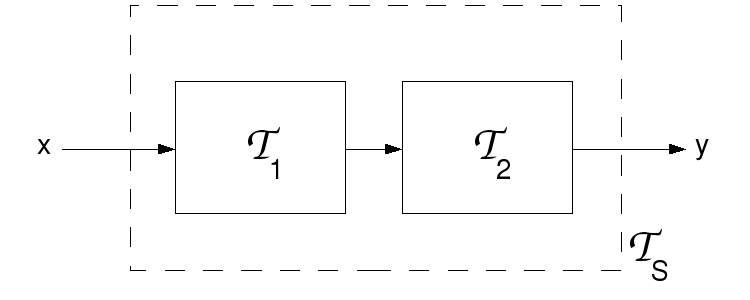
\includegraphics[width=7cm]{serie.png}\end{minipage}
\end{center}

\vskip 0.2cm
\noindent
Propietat: en general ${\cal T}_2 {\cal T}_1 \neq {\cal T}_1 {\cal T}_2$.

\item En \textbf{paral.lel}.
Donats dos sistemes ${\cal T}_1$ i ${\cal T}_2$, l'interconnexi\'o
en paral.lel de ${\cal T}_1$ i ${\cal T}_2$ d\'ona lloc a un nou sistema
${\cal T}_P$ tal que ${\cal T}_P={\cal T}_1 + {\cal T}_2$, \'es a dir:
\[
{\cal T}_P(x[n])={\cal T}_1(x[n]) + {\cal T}_2(x[n])
\]
\noindent
gr\`aficament:

\begin{center}
\begin{minipage}{6cm}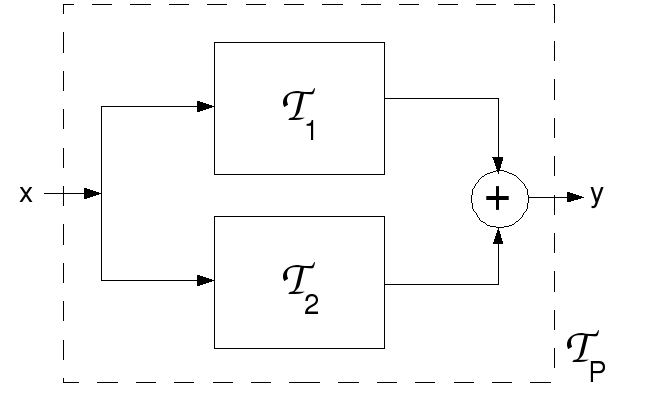
\includegraphics[width=6cm]{parallel.png}\end{minipage}
\end{center}

\vskip 0.2cm
\noindent
Propietat: ${\cal T}_1 + {\cal T}_2 = {\cal T}_2 + {\cal T}_1$.

\end{itemize}

\vskip 0.3 cm
\noindent
\textbf{An\`alisi de sistemes sineals i invariants en el temps (LTI)}
Els sistemes que s\'on a la vegada lineals i invariants en el temps es
denoten amb les sigles LTI (\textit{linear time-invariant}) i s\'on
especialment importants en Processament del Senyal perqu\`e
el seu funcionament es pot caracteritzar f\`acilment en funci\'o de la seva 
resposta a un senyal delta de Dirac.

\vskip 0.2 cm
\noindent
Sigui ${\cal T}$ un sistema LTI i sigui $x[n]$ un senyal d'entrada qualsevol.
Hem vist en el tema anterior que $x[n]$ es pot escriure en termes de la delta
de Dirac d'acord amb la f\`ormula $x[n]=\sum_{k=-\infty}^{+\infty} x[k] \delta[n-k]$,
de manera que la resposta del sistema a l'entrada $x[n]$ \'es:
\[
\begin{array}{ll}
y[n]& ={\cal T}(x[n])={\cal T} \left( \sum_{k=-\infty}^{+\infty} x[k] \delta[n-k] \right) = \\ \\
&= \text{(per linealitat)} = \sum_{k=-\infty}^{+\infty} x[k] {\cal T}(\delta[n-k]) = \\ \\
&= \text{(per invari\`ancia en el temps)}= \sum_{k=-\infty}^{+\infty} x[k] h[n-k]
\end{array}
\]
\noindent
on $h[n]={\cal T}(\delta[n])$, la resposta del sistema a una delta de Dirac.
$h[n]$ es coneix com \textbf{resposta impulsional del sistema}.

\vskip 0.2 cm
\noindent
Si observam el resultat anterior i recordam la definici\'o de convoluci\'o veurem que
\[
y[n]=x[n] * h[n]
\]

\noindent
\'Es a dir, \textbf{la sortida d'un sistema LTI \'es igual a la convoluci\'o
del senyal d'entrada per la resposta impulsional del sistema}. Per aquest motiu deim
que la resposta impulsional caracteritza totalment el sistema LTI. Si coneixem $h[n]$
podrem con\`eixer la resposta a qualsevol senyal d'entrada.

\vskip 0.2 cm
\noindent
Propietats dels sistemes LTI:
\begin{itemize}
\item Un sistema LTI \'es causal si i nom\'es si $h[n]=0 \quad \forall n < 0$.
\item Un sistema LTI \'es estable si  i nom\'es si $\sum_{n=-\infty}^{+\infty} |h[n]| < \infty$. 
\item La interconnexi\'o en s\`erie de dos sistemes LTI \'es commutativa, \'es a dir ${\cal T}_1 {\cal T}_2 = {\cal T}_2 {\cal T}_1$.
\end{itemize}


\vskip 0.2 cm
\noindent
Classificaci\'o dels sistemes LTI segons la duraci\`o de la seva resposta impulsional:
\begin{itemize}
\item Sistemes FIR (\textit{finite-duration impulsional response}).
S\'on aquells en qu\`e la resposta impulsional val zero fora d'un cert
interval de temps. En particular, per a un sistema FIR causal tenim que
\[
h[n]=0 \qquad \text{si } n < 0 \quad \text{i } n \geq M
\]
\noindent
per a algun valor de $M$ finit. De manera que la sortida d'aquest tipus de
sistemes es pot escriure com:
\[
y[n]=\sum_{k=0}^{M-1} x[k] h[n-k]=\sum_{k=0}^{M-1} x[n-k] h[k]
\]

\item Sistemes IIR (\textit{infinite-duration impulsional response}).
En aquest cas la resposta impulsional no s'anul.la fora de cap interval i
la sortida del sistema s'escriu com un sumatori infinit de valors.
\end{itemize}


\newpage
%\vskip 0.3 cm
\noindent
\textbf{Sistemes LTI descrits per equacions en difer\`encies finites}

\vskip 0.2 cm
\noindent
Els sistemes FIR s\'on \textit{realitzables} (es poden implementar amb un ordinador o circuit 
digital) ja que impliquen un nombre finit d'operacions i d'espais de mem\`oria.
En canvi, els sistemes IIR semblen irrealitzables ja que es necessiten, en principi,
infinites operacions i espai de mem\`oria. No obstant, hi ha un tipus de sistemes IIR, 
anomenats sistemes IIR \textbf{recursius} (o realimentats), que s\'on realitzables si involucren un nombre finit 
d'operacions.

En general, un sistema recursiu realitzable \'es aquell en qu\`e la seva sortida es pot escriure en funci\'o
d'un nombre finit de les entrades i de les sortides anteriors:
\[
y[n]=F( y[n-1], y[n-2], \cdots, y[n-N], x[n], x[n-1], \cdots, x[n-M]  )
\]

Un sistema es diu \textbf{no recursiu} si la seva sortida nom\'es dep\`en de les
entrades:
\[
y[n]=F( x[n], x[n-1], \cdots, x[n-M]  )
\]

Els sistemes FIR causals s\'on sistemes no recursius.


\vskip 0.3 cm
En aquest apartat estudiam com calcular de manera expl\'icita la sortida dels sistemes
recursius descrits per equacions de la forma:
\[
y[n]+\sum_{k=1}^N a_k y[n-k] = \sum_{k=0}^M b_k x[n-k]
\]
Aquest tipus d'equaci\'o rep el nom d'\textbf{equaci\'o en difer\`encies finites amb coeficients constants}.
$N$ s'anomena \textbf{grau} de l'equaci\'o.


\vskip 0.3 cm
La soluci\'o general d'aquesta equaci\'o es calcula de la forma seg\"uent:


\begin{enumerate}
\item la soluci\'o $y[n]$ s'escriu com la suma de dos termes
\[
y[n]=y_H[n]+y_P[n]
\]
\noindent
anomenats, respectivament, \textbf{soluci\'o homog\`enia} ($y_H$) i \textbf{soluci\'o particular} ($y_P$).

\item La soluci\'o homog\`enia \'es la soluci\'o de l'equaci\'o:
\[
y[n]+\sum_{k=1}^N a_k y[n-k] = 0
\]
\noindent
que rep el nom d'\textbf{equaci\'o homog\`enia}.

$y_H[n]$ es calcula de la seq\"uent manera:

\begin{enumerate}

\item escrivim l'\textbf{eq\"uaci\'o caracter\'istica} associada a l'eq\"uaci\'o
homog\`enia:
\[
\lambda^N+\sum_{k=1}^N a_k \lambda^{N-k} = 0
\]
\noindent
aquesta equaci\'o t\'e grau $N$.
\item calculam les arrels de l'eq\"uaci\'o caracter\'istica:
\[
\begin{array}{c}
\lambda_1 \text{ amb multiplicitat } r_1 \\ \\
\lambda_2 \text{ amb multiplicitat } r_2 \\ \\
\cdots \\ \\
\lambda_m \text{ amb multiplicitat } r_m
\end{array}
\]

\noindent
Es verifica que $r_1+r_2+\cdots+r_m=N$

\item per a cada arrel $\lambda_i$ amb multiplicitat $r_i$ de l'equaci\'o 
caracter\'istica tenim una soluci\'o parcial de l'equaci\'o homog\`enia:
\[
C_{i1} \lambda_i^n + C_{i2} n \lambda_i^n + \cdots + C_{i r_i} n^{r_i-1} \lambda_i^n
= \sum_{j=1}^{r_i} C_{ij} n^{j-1} \lambda_i^n
\]

\item la soluci\'o de l'equaci\'o homog\`enia s'obt\'e sumant totes les solucions parcials
\[
y_H[n]=\sum_{i=1}^m \sum_{j=1}^{r_i} C_{ij} n^{j-1} \lambda_i^n
\]

\item les constants $C_{ij}$ es calculen a partir de les 
\textbf{condicions inicials} del problema.

\end{enumerate}



\item La forma de la soluci\'o particular $y_P[n]$ dep\`en del tipus del senyal d'entrada $x[n]$:

\begin{tabular}{c|c}
Senyal d'entrada & Soluci\'o particular \\ 
$x[n]$, $n \geq 0$ & $y_P[n]$, $n \geq 0$ \\ 
($x[n]=0$ si $n < 0$) & ($y_P[n]=0$ si $n < 0$)\\  \hline \\
$(A_0+A_1 n + \cdots + A_k n^k) \alpha^n$ & $(B_0+B_1 n + \cdots + B_k n^k) n^M \alpha^n$ \\ \\
 & on $M$ \'es la multiplicitat de $\alpha$ com a soluci\'o de l'equaci\'o caracter\'istica \\
\hline
\\
$A \cos(\omega_0 n)$ & $B_1 \cos(\omega_0 n) + B_2 \sin(\omega_0 n)$ \\ \\
\hline
\\
$A \sin(\omega_0 n)$ & $B_1 \cos(\omega_0 n) + B_2 \sin(\omega_0 n)$ 
\end{tabular}

\noindent
\vskip 0.3 cm
Les constants $B_i$ es calculen per substituci\'o en l'equaci\'o en difer\`encies inicial.

\end{enumerate}



\vskip 0.4cm
\noindent
\textbf{Exemple:} Calculau la soluci\'o del sistema recursiu descrit per l'equaci\'o seg\"uent
considerant condicions inicials $y[k]=1$ per a tot $k < 0$.
\[
y[n]-5y[n-1]+6y[n-2]=u[n]
\]

\vskip 0.2cm
\noindent
Soluci\'o:
\begin{enumerate}
\item $y[n]=y_H[n]+y_P[n]$
\item $y_H[n]$:
\begin{enumerate}
\item equaci\'o homog\`enia: $y[n]-5y[n-1]+6y[n-2]=0$ (grau 2)
\item equaci\'o caracter\'istica: $\lambda^2 - 5 \lambda + 6 =0$
\item arrels de l'equaci\'o caracter\'istica: $3$ i $2$
\item $y_H[n]=C_1 3^n + C_2 2^n$
\end{enumerate}
\item $y_P[n]$:
\begin{enumerate}
\item $x[n]=A u[n]$, amb $A=1$ (polinomi de grau 0)
\item $y_P[n]=B u[n]$
\item substituint a l'equaci\'o inicial:
\[
\begin{array}{l}
y_P[n]=B u[n] \\
y_P[n-1]=B u[n-1] \\
y_P[n-2]=B u[n-2] \\
y_P[n]-5y_P[n-1]+6y_P[n-2]=u[n] \quad \Rightarrow Bu[n]-5Bu[n-1]+6Bu[n-2]=u[n]\\
\text{per a $n >= 2$ la resposta s'estabilitza i tenim:} \qquad B-5B+6B=1 \quad \Rightarrow B=\frac{1}{2}
\end{array}
\]
\item per tant: $y_P[n]=\frac{1}{2} u[n]$
\end{enumerate}

\item Soluci\'o completa: $y[n]=C_1 3^n + C_2 2^n+\frac{1}{2} u[n]$

\item C\`alcul de $C_1$ i $C_2$:
\begin{enumerate}
\item de l'equaci\'o inicial i aplicant les condicions inicials ($y[k]=1$ si $k < 0$):
\[
\begin{array}{l}
y[0]-5y[-1]+6y[-2]=u[0] \quad \longrightarrow \quad y[0]=5-6+1=0 \\
y[1]-5y[0]+6y[-1]=u[1] \quad \longrightarrow \quad y[1]=0-6+1=-5 
\end{array}
\]
\item de la soluci\'o trobada:
\[
\begin{array}{l}
y[0]=C_1 3^0 + C_2 2^0+\frac{1}{2} u[0] \quad \longrightarrow \quad y[0]=C_1+C_2+\frac{1}{2} \\ 
y[1]=C_1 3^1 + C_2 2^1+\frac{1}{2} u[1] \quad \longrightarrow \quad y[1]=3C_1+2C_2+\frac{1}{2} \\ 
\end{array}
\]
\item resolent el sistema d'equacions que plantejen les anteriors equacions: $C_1=-\frac{13}{2}$, $C_2=7$.

\end{enumerate}
 
\item Soluci\'o final: $y[n]=-\frac{13}{2} \cdot 3^n + 7 \cdot 2^n+\frac{1}{2} u[n]$

\end{enumerate}



\vskip 0.4cm
\noindent
\textbf{Respostes lliure i for\c{c}ada d'un sistema} 

\vskip 0.2 cm
\noindent
La resposta total d'un sistema es pot escriure com la suma de dos termes
\[
y[n]=y_{zi}[n]+y_{zs}[n]
\]

\noindent
on $y_{zi}$ s'anomena \textbf{resposta zero-input}, resposta lliure o resposta natural
del sistema. \'Es la resposta que s'obt\'e quan l'entrada \'es nul.la i coincideix amb
la soluci\'o homog\`enia de l'equaci\'o en difer\`encies ($y_{zi}[n]=y_H[n]$).

\noindent
$y_{zs}$ rep el nom de \textbf{resposta zero-state} o resposta for\c{c}ada del sistema
i \'es la resposta que s'obt\'e davant un senyal d'entrada quan les condicions inicials s\'on
nul.les (sistema en rep\`os o relaxat). Coincideix amb la soluci\'o del sistema
quan les condicions inicials s\'on nul.les ($y_{zs}[n]=y[n]$, amb $y[n]=0$ per $n < 0$).

\vskip 0.4cm
\noindent
\textbf{Resposta impulsional d'un sistema recursiu} 

\vskip 0.2 cm
\noindent
La resposta impulsional $h[n]$ d'un sistema LTI es defineix com la resposta
del sistema a un senyal delta de Dirac. En el cas d'un sistema descrit per una
equaci\'o en difer\`encies $h[n]$ coindideix amb la resposta del sistema quan
$x[n]=\delta[n]$ i les condicions inicials s\'on nul.les: 
\[
h[n]=y[n] \qquad \text{quan} \quad x[n]=\delta[n] \quad \text{i} \quad y[n]=0 \text{ per } n < 0
\]

\noindent
a m\'es, com $x[n]=\delta[n]$, resulta que $y_P[n]=0$ i per tant $y[n]=y_H[n]$.



\vskip 0.4cm
\noindent
\textbf{Estructures per a la realitzaci\'o de sistemes LTI descrits per equacions en difer�ncies} 

\vskip 0.2 cm
\noindent
El diagrama de blocs corresponent a l'equaci\'o en difer\`encies

\[
y[n]=-\sum_{k=1}^N a_k y[n-k] + \sum_{k=0}^M b_k x[n-k]
\]

\noindent
es mostra en la figura \ref{blocsLTI}-(a). Per la propietat 
conmutativa de la connexi\'o en s\`erie dels sistemes LTI
(${\cal T}_1 {\cal T}_2 = {\cal T}_2 {\cal T}_1$), aquest diagrama
\'es equivalent al de la figura \ref{blocsLTI}-(b), que
\'es equivalent al de la figura \ref{blocsLTI}-(c). En aquest 
darrer diagrama el nombre d'operacions de retard \'es menor que
en els diagrames anteriors, per la qual cosa es considera que
la realitzaci\'o del sistema \'es m\'es eficient. La realitzaci\'o de l'esquerra
s'anomena \textbf{forma directa} del sistema mentre que la de
la dreta es diu \textbf{forma can\`onica}.

\begin{figure}[htbp]
\begin{center}
\begin{tabular}{cc}
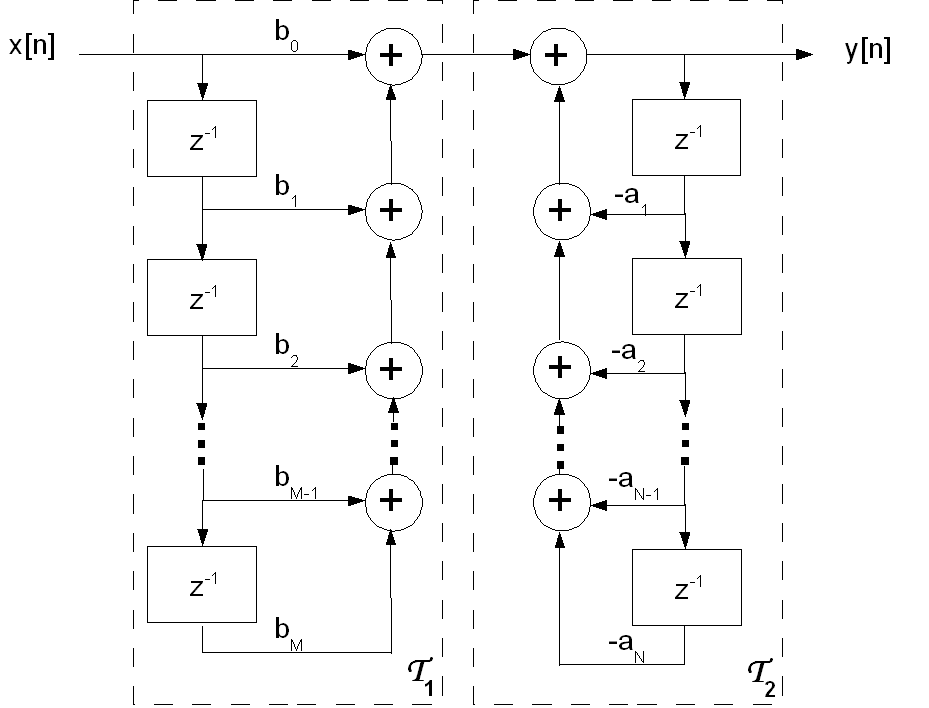
\includegraphics[width=8cm]{formadirecta.png} &
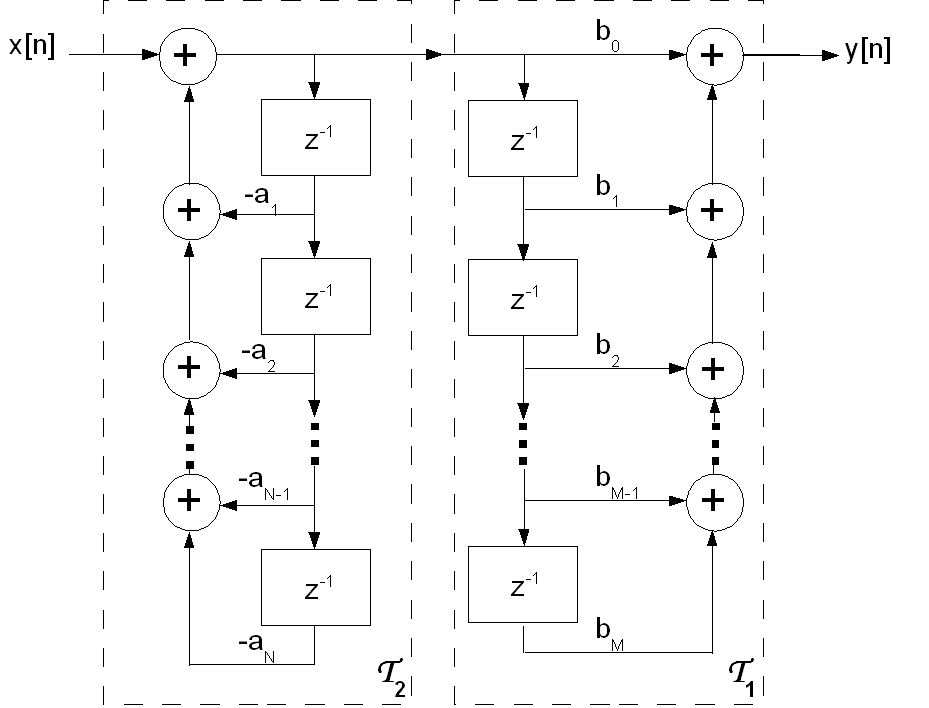
\includegraphics[width=8cm]{formacommutada.png} \\ \\
(a) & (b) 
\end{tabular}
\begin{tabular}{c}
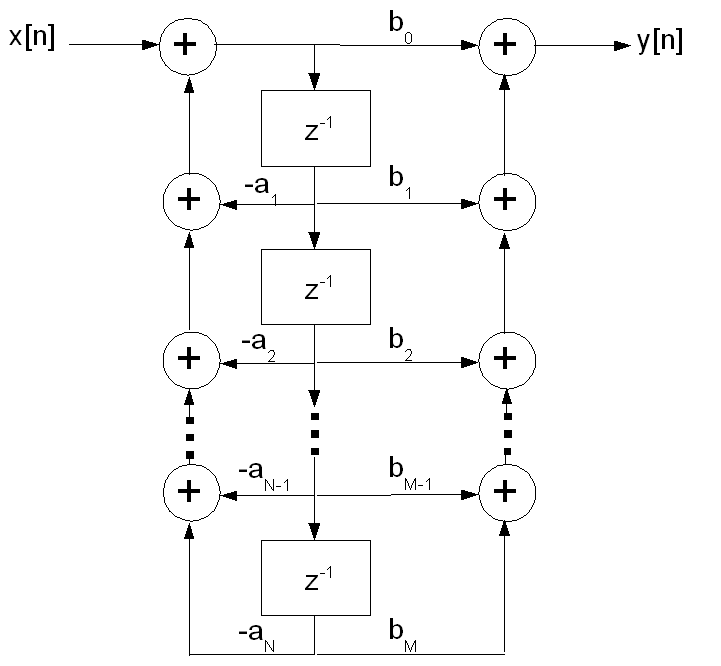
\includegraphics[width=7.5cm]{formacanonica.png} \\ \\
(c)
\end{tabular}
\end{center}
\caption{(a) forma directa. (b) commutaci\'o de les estructures
del diagrama anterior. (c) forma can\`onica.}
\label{blocsLTI}
\end{figure}


\end{document}

